\section{Research Questions and Hypothesis}
    
  {\bf $H_{0}$: Human properties have no influence in users choice of graphical passwords} 

  {\bf $H_{1}$: Users choice of graphical passwords are influenced by the human properties of the user}

\section{Research Strategy}

  \subsection{Selection of Research Strategy and Data Collection}

    In this thesis, the selected research strategy is a Servey. To be able to answer the hypothesis there is a need for obtain data from a large group of people in a standardarized and systematic way. This will provide a wide and inclusive coverage of people so the results from the data collection are likely to be representative for a wider population. 

    When selecting survey as a research strategy, a questionaire would be a good fit for the quantitative data collection. The data properties that is selected are indicating that data needs to be collected ``world wide'', and cannot be collected face-to-face due to the lack of time and resources. For analyzing patterns in the data, a big amount of data needs to be collected. The questionaire will be distributed over the internet and will be helpful in the data collection process to get a sampling frame that is large enough. Data collection with pen and paper are to time consuming and would not be manageable with the time available for data collection and analysis in the spring. When analyzing data, it is also nessesary to have the data in a standardized format. A questionarie is supporting a stadarized format, and with a online tool it will be easy to extract the data in a standarized format for the analysis. This will provide the possibility to use automatically analysis tools without to much use of time with manually work.

    A limitations of the chosen approach is that it does not support control of the participants because the questionaire is distributed over web, and users are not hanpicked. Since the data collection is distributed over web, there is not possibility for judge the accuracy and honesty of peoples responses. Despite the limitations, this is chosen due to the amout of data needed for the analysis, as well as the lack of time for choosing other approaches like interviews and other observation techniques. 

    The detailed design of the questionarie will be described in section 4.3.

  \subsection{Data Requirements}
  
  It is important to analyse what kind of human factors that may inpact users choice of graphical passwords on mobile devices. We must carefully consider which human properties we want to collect in order to get a consise collection of data that can be analyzed, and further give us answer to our hypoteses. This analysis will be a review of human properties that this study find relevant to the hypotheis. As a result of this analysis, a narrowed selection of the listed human properties will further be included in the data collection.  

  \begin{itemize}
    \item {\bf Age:} A group of people within a certain age group may have different risk awareness. A person with a age between 30-40 and a person with a age below 20 may have different concerns with security. A person in the age between 30-40 may use their phone to perfrom task with a high security risks like manking and job releated tasks, while a person with a age below 20 may not have the same security awareness because of the different use of mobile devices.
    \item {\bf Gender:} Psychological studies have reported that males are more likely to take risks than females \cite{Byrnes}. When looking at peoples choice in patterns can probabliy be analysed based on gender. In the litterature review there was no reported results found on genders risk awareness in information security. By analysing peoples choice of patterns based on users gender might be related to the psychological studies.
    \item {\bf Nasjonality:} 
    \item {\bf Language preference:}
    \item{\bf Occupation:}
    \item {\bf Profession:} The profession of a person may say something about a persons knowledge and background. When looking at profession, a person with a profession in IT may be more certain about the security aspects than people in other professions. 
    \item {\bf Left- or right handed:} An interesting property of humans is the fact that people write with either left or right hand (and sometimes both). This property can influence the way that a person are helding the phone and may inpact the way that a person is making a pattern. In the litterature review it was not found any studies that have studied the impact of patterns or passwords based on this property. An interesting analysis can be done by looking at this property along with the size of the mobile device. Published research \cite{Uellenbeck} found that over 40\% of interest in a study started their Android pattern by starting in the top left corner, but did not record the hand used when making the pattern. My hypotehis is that a left handed person may be using the left hand while interacting with the phone, making the probability for starting in the right upper corner bigger. This have never been tested before and need further research before making a statement. 
    \item {\bf Reading/writing orientation:} In different cultures, there is a difference in the reading and writing direction. Cultures from Europe and America is normally writing and reading horizontally from left to right, but there are other cultures that do otherwise. Traditionally, Chinese, Japanese, and Korean are writing text vertically in columns from top to bottom, from right to left. Another writing orientation is horizontal from right to left that are used in arabic cultures. Today, the vertical orientation from top to bottom is often in a horizontal way due to the influence of English and the increased computerized typesetting, but both ways are still in use. There are research that have reported that the writing orientation are affecting the visual attention and memory \cite{Chan}. They forund that the reading orientation affected the way a person would memorize objects. They reported that English and Chinese speakers tended to remember an image that appeared in the top, left-hand side of the screen and the Taiwanese speakers tended to remember the images in the upper right-hand side of the screen. The interesting aspect of this reading and writing orientation is to see if people from different cultures are choosing different patterns due to their writing orientation.
    \item {\bf Hand size:} Smartphones today tends to get bigger and bigger in size. An interesting analysis could be done by looking at a users choice of patterns based on size of hands and size of mobile phone where a patterns is made. By looking at a situation were a person with a small hand and a big mobile device, it may be hard to reach certain areas on the screen by holding a device in one hand and therefore inpact the patterns made. 
  \end{itemize}

  \begin{figure}[H]
    \centering
    \subfigure{
      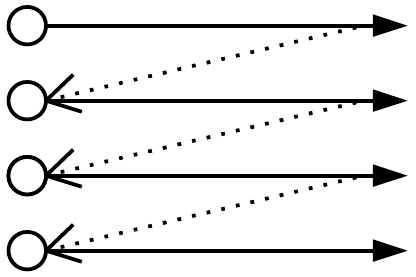
\includegraphics[scale=0.25]{pics/leftright.png}
    }
    \subfigure{
      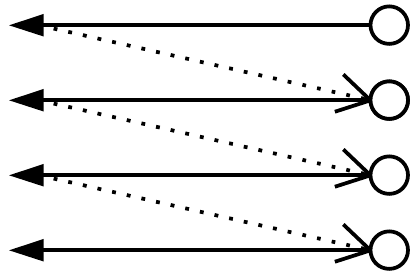
\includegraphics[scale=0.25]{pics/rightleft.png}
    }
    \subfigure{
      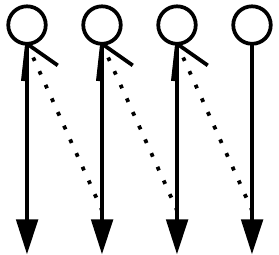
\includegraphics[scale=0.27]{pics/topbottom.png}
    }
    \caption{Writing orientatio: 1) Horizontally Left-to right, 2) Horizontally Right-to-left 3) Vertically Right-to-left}
  \end{figure}

  \todo{Vil det være lurt å spørre om innhold på mobil og bruksområde? Vil det ha noe utslag på feks styrke på mønster?}
  \todo{Tenke fremover: hvilke mønster vil jeg se etter? Hvilke resultater kan forekomme som kan kreve ekstra data for videre analyse?}

  \subsection{Sampling Frame and Technique}

    \todo{Er der her jeg skal nevne hvem jeg ønsker å samle inn svar fra (sampling frame)?}
    
    The survey type is categorized as ``non-probability sampling'' and the chosen sample technique is ``self-selection strategy''. This is chosen due to time and cost estimates, and the lack of control of participants. A Purposive sampling technique would maybe provide a more uniformly collection of people, but it is hard to control the participants when the questionaire is distributed on the web. The self-selection strategy will collect data from any respondants, and will be helpful when there is big population with potetial respondants. The self-selection is a useful technuiqe when we are not able to directly contact the potential respondants. When people select themselves for research, it might indicate that they have a strong feeling on the subject, or becuase they think it will bring them persenal benefit or approval. 

  \subsection{Response Rate and Non-responses}
    \begin{itemize}
      \item Response rates of 10\% are not uncommon
      \item I need to look for a strategy that may increase the number of responses
      \item If I suspect that certain types of people in my sample will be less willing to respond, I could deliberatley include more of that type in my sample so I can asure that I recive the number of respondants that I need. Maybe go face-to-face if a group of people may be less willing to participate. 
      \item Need to find characteristics of people that have noot answeard to make a discussion of why they didnt (maybe they are not representative), or wether their non-response is meaningful in its own right, or wheter their lack of responses has resulted bias in my final sample.
      \item 
      \end{itemize}

  \subsection{Sample Size}
    I need to decide how big I want my final sample to be, taking into account my best estimate of the likely non-response rate of participants. 
    Good rule of thumb is to have at least 30. For a target population of 1 million or more, I would probably nedd 1000. 

    The Internet offers researchers the possibility of accessing many people across the world cheaply and quickly. Not everyone have internet access, and that need to be considered in the design. Maybe they are not a targeted group since this is a mobile focus.

